% This is samplepaper.tex, a sample chapter demonstrating the
% LLNCS macro package for Springer Computer Science proceedings;
% Version 2.21 of 2022/01/12
%
\documentclass[runningheads]{llncs}
%
\newcommand{\False}{\type{False}}
\newcommand{\True}{\type{True}}
\usepackage{changepage}
\usepackage{hyperref}
\newenvironment{myindent}{\begin{adjustwidth}{1cm}{}}{\end{adjustwidth}}

\usepackage{listings}
\usepackage{lipsum}
\usepackage{courier}
\usepackage{color}
\lstset{basicstyle=\footnotesize\ttfamily,breaklines=true}
\lstset{frame=single}


\usepackage[T1]{fontenc}
% T1 fonts will be used to generate the final print and online PDFs,
% so please use T1 fonts in your manuscript whenever possible.
% Other font encondings may result in incorrect characters.
%
\usepackage{graphicx}
% Used for displaying a sample figure. If possible, figure files should
% be included in EPS format.
%
% If you use the hyperref package, please uncomment the following two lines
% to display URLs in blue roman font according to Springer's eBook style:
%\usepackage{color}
%\renewcommand\UrlFont{\color{blue}\rmfamily}
%
\begin{document}
%
\title{Formalizing the unexpected hanging paradox: a classic surprise} %\thanks{Supported by organization x.}}
%
%\titlerunning{Abbreviated paper title}
% If the paper title is too long for the running head, you can set
% an abbreviated paper title here
%
\author{Polina Vinogradova\inst{1}\orcidID{0000-0003-3271-3841} }
% \and
% Second Author\inst{2,3}\orcidID{1111-2222-3333-4444} \and
% Third Author\inst{3}\orcidID{2222--3333-4444-5555}}
%
\authorrunning{Polina Vinogradova}
% First names are abbreviated in the running head.
% If there are more than two authors, 'et al.' is used.
%
\institute{IOG
\email{polina.vinogradova@iohk.io}}
%
\maketitle              % typeset the header of the contribution
%
\begin{abstract}

  In this work, we define a novel approach to the formalization of the
  unexpected hanging paradox, sometimes called the surprise examination paradox,
  mechanized in the Coq Proof Assistant.
  This paradox requires the definition of the notion of
  a \emph{surprise} event, which, for the purposes of this paradox, is usually interpreted as
  the inability to predict what day a specific event takes place. As in existing work,
  the use of constructive logic allows us to distinguish between possibility and
  certainty.
  We make the observation that an inevitable, but unexpected, event requires there being strictly
  more than one possible day on which it can occur, and define surprise accordingly. We
  formalize the paradox using this interpretation of surprise.
  We observe that our paradox specification
  can be instantiated equally well in both constructive and classical logics.
  The classical instantiation of our definition lets us formally make the same intuitive
  conclusions as the constructive definition, and as
  existing work which uses self-referential predicates.
  We assert that this offers a satisfying resolution to the paradox in accordance with
  our intuition.
  We compare our definition to an existing, weaker, interpretation of surprise,
  giving an analysis of how it interplays with the use of constructive logic.

\keywords{surprise examination \and paradox \and unexpected hanging \and formalization \and Coq \and constructive logic.}
\end{abstract}
%




\section{Introduction}

The unexpected hanging paradox, also known as the surprise examination paradox,
is a logical paradox introduced in the the Mind philosophical journal in 1948 \cite{original},
and popularized by the Scientific American Mathematical
Games column author Martin Gardner, discussed in his work \cite{diversions}.
It describes the notion of a future event that
is both certain, and not possible to predict the exact day of occurrence of. It is
formulated as follows: \newline

\begin{myindent}
  A judge tells a condemned prisoner that he will be hanged at noon on one weekday
  in the following week but that the execution will be a surprise to the prisoner.
  He will not know the day of the hanging until the executioner knocks on his cell door at noon that day.

  Having reflected on his sentence, the prisoner draws the conclusion that he will
  escape from the hanging. His reasoning is in several parts. He begins by concluding
  that the "surprise hanging" cannot be on Friday, as if he has not been hanged by
  Thursday, there is only one day left – and so it won't be a surprise if he's hanged on
  Friday. Since the judge's sentence stipulated that the hanging would be a surprise
  to him, he concludes it cannot occur on Friday.

  He then reasons that the surprise hanging cannot be on Thursday either, because
  Friday has already been eliminated and if he has not been hanged by Wednesday noon,
  the hanging must occur on Thursday, making a Thursday hanging not a surprise either.
  By similar reasoning, he concludes that the hanging can also not occur on Wednesday,
  Tuesday or Monday. Joyfully he retires to his cell confident that the hanging will
  not occur at all.

  The next week, the executioner knocks on the prisoner's door at noon on Wednesday –
  which, despite all the above, was an utter surprise to him. Everything the judge said came true. \newline
\end{myindent}

 Existing formalization efforts attempt to address questions like "how can we formally
define surprise within the conditions of this paradox?", "where is the flaw in the
reasoning of the prisoner?" and "was it contradictory for the prisoner to have been
hanged on Wednesday?". There is work on tackling these questions in multiple
different branches of philosophy and mathematics.
An extensive review of the existing approaches is given in \cite{extensivereview}.

The definition of surprise as the inability to deduce beforehand the date of the test
was first introduced in \cite{prediction}. A statistical approach to the problem
of prediction in this context is discussed in \cite{statistical}.
A proposed solution in the field of epistemology with the use of modal
logic, is presented in \cite{modalepistemic}. An approach involving
Kripke semantics, employing the notion of persuasion, is in \cite{kripkemodal}.

The use of constructive logic,
e.g., appealing to G\"{o}del's incompleteness, was first applied to the
paradox in \cite{goedelized}, then in \cite{godelinconsistent}, and most recently
in \cite{constructive} \cite{nonpredet}. The first two rely on reasoning via the provability operator $\mathsf{Pr}$ to indicate
a possibly non-classical statement, while the others assume the underlying logic to be itself
constructive. This approach aligns most closely with ours.

The work \cite{fourpossible} investigates the relation between the conclusions
of the non-classical logic approaches and those from epistemology, as well
as presenting four distinct approaches to formalizing the paradox, from which
we take inspiration.

Here, we give formal and mechanized descriptions of related but distinct aspects of the
paradox: the conditions of the
paradox, and a predicate that can be used to make judgements about the hanging day
in accordance with the paradox constraints. We note that such a predicate
can be instantiated both classically and intuitionistically. With the
right definition of "knowledge of the hanging day", either option allows us
to make consistent judgements, as well as judgements about inconsistencies,
which are similar in content to the self-referential formalization presented
in \cite{godelinconsistent}.

We take as our base assumption that the constraints of the paradox are
fixed and correctly conveyed to the prisoner. This includes a fixed, a-priori selected execution date.
Like the works we cited above, we do all our reasoning in constructive logic,
leaving room for uncertainty, or possibility, by
dropping the law of excluded middle. We additionally, make the assumption that
the prisoner is able to continue drawing conclusions about the paradox on days
after the hanging occurs. This is actually more in line the surprise examination version of this paradox,
wherein the students are both surprised and alive after the exam happens.

In our formalization we do not make use of modal or temporal logic
(which is the approach in \cite{modalepistemic}).
Instead, we take advantage of the expressivity of the dependently typed logic of Coq to
build our formalization, parametrized by weekdays in the
appropriate way.
Investigating the possibility of re-defining our
dependently-typed functions as clauses in modal logic remains the subject of future work.

We chose to use a proof
assistant (Coq, see \cite{coqmanual}) to take a more high-assurance look at the
interplay between the seemingly simple conditions of this conundrum.
There is precedent for the use of proof assistants to tackle philosophical
investigation, with the most striking and recent example
being a refinement of Kant's categorical imperative \cite{categoricalkant}.

  The contributions of this paper are as follows:

  \begin{itemize}
    \item[(i)] A definition of surprise, together with the paradox
    constraints, without self-reference,
    Sections \ref{sec:lack} \ref{sec:constraints}, reflecting
    the following natural language statement: "a hanging has not occurred on or before a given day,
    and there exist at least two distinct future days on which a hanging
    is possible". We
    also give an analysis of how this definition aligns with our intuition;

    \item[(ii)] The construction of a three-parameter predicate returning a proposition about
    whether or not a hanging happens on \emph{a given day}, given that we know whether or not a hanging
    happened on days up and including the parameter day \emph{today}, and a day on which the hanging
    \emph{actually happens}, see Section \ref{sec:predicate};

    \item[(iii)] A proof that a classical instantiation of the predicate in (ii)
    is in accordance with our paradox specification, see Section \ref{sec:constraints};

    \item[(iv)] A proof that a hanging having not occurred by Thursday does not let
    us conclude whether one will occur Friday or not, regardless of the specific
    definition of the predicate in (ii), Section \ref{sec:constraints};

    \item[(v)] An alternate, weaker formalization of surprise (Section \ref{sec:one}). We give an analysis of how
    our definition compares to this one, and why it gives us insufficient reasoning
    power in the case that the surprise reasoning predicate is non-classical, but
    in the case that it is classical, allows us to reason ourselves out of the hanging entirely by concluding
    a sure-thing Friday hanging on Thursday;

    \item[(v)] An associated mechanization, in the Coq Proof Assistant, of the formal
    definitions and proofs in (i)-(v).
  \end{itemize}

  For our code, see \url{https://github.com/polinavino/unexpected_hanging/blob/master/unexpected_hanging.v}.

\section{Mechanizing and the Paradox}
\label{sec:form}

Coq is a proof assistant that offers a dependently typed formal language.
It is capable of verifying formal user-defined proofs of propositions, as well as supporting
the automation of certain kinds of proofs. The choice of Coq, as opposed to another
proof assistant such as Agda, was based largely on the authors' familiarity with the system,
as any dependently typed proof verifier that supports constructive logic
would serve just as well for the purposes of this mechanization.

To formalize the paradox, we need to reason about days of the week on which
the paradox could happen, so we
begin by constructing a type {\tt weekDay}, the terms of which are week days:

\begin{lstlisting}[mathescape=true]
  Inductive weekDay : Type :=
    | monday : weekDay | ... | friday : weekDay.

  Inductive weekAndBefore : Type :=
    | dayBefore : weekAndBefore | someWeekDay : weekDay $\to$ weekAndBefore.
\end{lstlisting}

We define the type {\tt weekAndBefore}, which represents all the weekdays in
the type above, plus the Sunday that comes before. The purpose of this type is to
represent all the days on which one can consider the possibility of surprise,
differentiating it from the subset of days on which the hanging can occur. We
also define comparison function {\tt <}, which computes
whether a given {\tt td : weekAndBefore} is before {\tt d : weekDay},
following real-life weekday logic, e.g. Sunday is before Monday.

It is important to emphasize here that $=,~\geq,~<$ are all \emph{decidable}
comparison functions on days --- purely as a consequence of considering weekdays
as totally ordered entities, even in constructive logic. Any predicates
formulated solely out of those comparisons together with logical connectives are also decidable,
with the implication that provability, knowledge, and truth are all the same for such predicates,
leaving no room for uncertainty.
Therefore, solutions of the paradox constructed out of only such decidable predicates (e.g. \cite{godelinconsistent})
are operating in classical logic.

For this reason we define a (for now) abstract function, which specifies a subset of
days of the week on which a hanging occurs.

\begin{lstlisting}[mathescape=true]
  Variable hangingOnDay : weekDay $\to$ Prop.
\end{lstlisting}

We discuss, in Section \ref{sec:predicate}, what properties and additional parameters of
such a function ensure that it conforms to the constraints of the paradox.
Next, we define a predicate that formalizes the notion that no hanging has occurred
yet (up to and including the parameter day {\tt td}, representing \emph{today}).
This says that for any day {\tt d}, if it is before today {\tt td}, no hanging
happened on {\tt d}:

\begin{lstlisting}[mathescape=true]
  Definition noHangingYet (td : weekAndBefore) :=
    $\forall$ d, td $\geq$ d $\to$ $\neg $ hangingOnDay d.
\end{lstlisting}

We use the double negation {\tt $\neg \neg$ hangingOnDay d} to formalize the statement that it is
not possible to disprove that a hanging occurs on day {\tt d}. That is, a hanging
is \emph{possible} on a given day.

\section{Uniqueness of hanging. }
\label{sec:unique}

Uniqueness of the hanging day plays an important role in the definition of surprise.
We define the predicate {\tt uniqueHanging} formalizing that "after a given day {\tt td},
there can be at most one day on which a hanging occurs". So,
{\tt uniqueHanging dayBefore} states this about the entire week.

\begin{lstlisting}[mathescape=true]
  Definition uniqueHanging (td : weekAndBefore) :=
    $\forall$ d d', td $<$ d $\wedge$ td $<$ d' $\to$
    hangingOnDay d $\to$ hangingOnDay d' $\to$ d = d'.
\end{lstlisting}

The constraint, {\tt uniqueHanging}, that
a \emph{provable} hanging day is unique is, in fact, equivalent to the constraint
that a \emph{possible} hanging day is unique. Negation of uniqueness
is also implied by a stronger statement, {\tt twoPossible}, which explicitly
requires the presence of at least two possibilities for the hanging date.
Note here also that this reasoning does not rely on any additional knowledge about
the hanging predicate or the real day of the hanging.

\begin{lstlisting}[mathescape=true]
  Definition uniqueMaybe (td : weekAndBefore) :=
    $\forall$ d d',
    td $<$ d $\wedge$ td $<$ d' $\to$
    $\neg~\neg$ hangingOnDay d $\to$
    $\neg~\neg$ hangingOnDay d' $\to$
    d = d'.

  Lemma uniqueMaybeEqv (td : weekAndBefore) :
    uniqueHanging td $\leftrightarrow$ uniqueMaybe td.

  Definition twoPossible (td : weekAndBefore) :=
    $\exists$ d d', td $<$ d $\wedge$ td $<$ d' $\wedge$ d $\neq$ d'
    $\wedge$ $\neg \neg$ hangingOnDay d $\wedge$ $\neg \neg$ hangingOnDay d'.

  Lemma twoNotUnique : $\forall$ td,
    twoPossible td $\to$ $\neg$ uniqueHanging td.
\end{lstlisting}

The proof of this lemma relies on the decidability of
{\tt d = d'}, together with modus tollens. This result seems wrong --- we would expect a hanging to be
unique --- it's implicit in the description of the paradox. However, our definition of
surprise, in fact, requires the non-uniqueness of a \emph{future} hanging. If a hanging
has already occurred in the \emph{past}, we must still ensure that no additional hanging
can happen in the future, making a past hanging unique.

\section{A lack of surprise}
\label{sec:lack}

Surprise is a hard concept to address, so we try to define, instead, what it means to be certain about
when a hanging happens, given a collection of days on which it can happen.
We define what it means for us to \emph{know} that a hanging happened before today {\tt td}:

\begin{lstlisting}[mathescape=true]
  Definition knowHanging (td : weekAndBefore) :=
    ($\exists$ d, td $\geq$ d $\wedge$ hangingOnDay d) $\wedge$ (uniqueHanging dayBefore).
\end{lstlisting}

For this predicate to be true, the function {\tt hangingOnDay} must be provably \texttt{True}
for exactly one day {\tt d} of the entire week, and {\tt False} for all other weekdays, and this day {\tt d} is
before or on {\tt td}.
This predicate {\tt knowHanging} should hold exactly when a hanging has already happened
before today.

Now, let us consider the negation of these two conditions for days {\tt d} after {\tt td}:

\begin{lstlisting}[mathescape=true]
  Definition dontKnowHanging (td : weekAndBefore) :=
    $\neg$ (($\exists$ d, td $<$ d $\wedge$ hangingOnDay d)
      $\wedge$ (uniqueHanging dayBefore)).
\end{lstlisting}

Representing that either there is no hanging, or it is not unique. Assuming no
hanging has yet happened, this expresses surprise fairly
well, however, it allows for the possibility that no hanging happens at all in the
rest of the week, which should only be true if one had occurred before {\tt td}.
So, we must add to this definition a constraint that if we are able to prove that no
hanging happens this week, we have proven {\tt False} (we will separately handle the case for when
a hanging did already happen).

Note here that while we want to say that on each future day {\tt d}, proving a hanging
occurrence should not be possible (i.e. {\tt $\neg$ hangingOnDay d}), adding this to
our definition will allow us to
prove that no hanging happens at all.
That is, the proposition that no hanging happens the entire week implies that no
hanging is even possible, as \newline

{\tt $\neg$ hangingOnDay d $\to$ $\neg$ ($\neg~\neg$ hangingOnDay d)} \newline

This is inconsistent with the intuition of the paradox.

We notice that both {\tt uniqueHanging td} and its negation are trivially
satisfied whenever {\tt $\neg$ ($\exists$ d, td $<$ d $\wedge$ hangingOnDay d)}. For this
reason we use the stronger {\tt twoPossible td} in our definition of surprise,
which contradicts the possibility of there not being a hanging at all, and
guarantees two possible days.

So, regardless of when the hanging actually happens, we define what it means
for surprise to being possible after {\tt td} as

\begin{lstlisting}[mathescape=true]
  Definition surprise (td : weekAndBefore) :=
    (noHangingYet td) $\wedge$ (twoPossible td).
\end{lstlisting}

\section{The hanging predicate}
\label{sec:predicate}

According to the definition of the paradox, a Wednesday hanging satisfies
the constraints. However, the spirit of the paradox seems to suggest there is nothing
special about a Wednesday hanging. Here, we explain how to parametrize our predicates
by different possible hanging days.

We already parametrize the function {\tt surprise} by today {\tt td},
representing our inability to predict a hanging day (i.e. choose a unique hanging day)
after {\tt td}. The function {\tt surprise} builds propositions
about whether a hanging day happened on some day {\tt d} by using the
predicate {\tt hangingOnDay}. We note that this predicate must actually be a different
predicate depending on what day {\tt td} is as well, since we must vary it to
indicate that we always have full knowledge of all days before today, as well as full
knowledge of the entire week whenever the actual hanging day has passed.
So, all in all, we are interested in a function \newline

{\tt hangingOnTodayIsReasoningAbout hang td d : Prop} \newline

that satisfies the paradox constraints. It has three parameters:

\begin{itemize}
  \item[(i)] {\tt hang : weekDay} is the day on which the hanging actually occurs.
  Once today is or after this day, surprise should no longer be possible, but the paradox
  conditions may not be violated);
  \item[(ii)] {\tt td : weekAndBefore}, which is the day that is "today", i.e. the day
  on which the prisoner is making the judgement about the hanging day. For each day up to and including today
  the proposition about whether a hanging has occurred or not is classical;
  \item[(iii)] {\tt d : weekDay}, the day about which the prisoner is making the judgement of whether a hanging occurred on this day or not (e.g.
  tomorrow), but should not be able to prove or disprove the occurrence of a hanging on,
  unless this day is prior to {\tt td}.
\end{itemize}

Such a parametrized predicate replaces the previous {\tt hangingOnDay} predicate
in our definitions.
To accommodate this change, we also parametrize all
other predicates used in the definition, e.g. {\tt noHangingYetparam hangingOn hang td}.

\section{Paradox statement}
\label{sec:constraints}

We finally give the full statement of the constraints to be placed by the description of the paradox on the
hanging predicate {\tt hangingOnTodayIsReasoningAbout} discussed above.

\begin{lstlisting}[mathescape=true]
  Definition twoPossiblePRDXparam
      (hangingOn : weekDay $\to$ weekAndBefore $\to$ weekDay $\to$ Prop)
      (hang : weekDay) (td : weekAndBefore) :=
    (td $\geq$ hang $\wedge$ (hangingOn hang td hang)
        $\wedge$ uniqueHangingparam (hangingOn hang td) dayBefore)
    $\vee$
    (td $<$ hang $\wedge$ noHangingYetparam td
        $\wedge$ twoPossibleparam (hangingOn hang td) td).
\end{lstlisting}

We want to define a {\tt hangingOnTodayIsReasoningAbout} such that
the following lemma holds true:

\begin{lstlisting}[mathescape=true]
Lemma hangingFuncOk : $\forall$ hang td,
    $\neg$ (td = (someWeekDay thursday) $\wedge$ hang = friday) $\to$
    twoPossiblePRDXparam
        (hangingOnTodayIsReasoningAbout hang td) td.
\end{lstlisting}

We explicitly exclude being surprised
on Thursday by a Friday hanging, as it appears to legitimately be a situation devoid
of surprise (see discussion below).
The statement of the paradox can be interpreted as follows: \newline

\begin{myindent}
  The executioner plans the hanging to be on the
  day {\tt hang}. He tells the prisoner that in order to, on each day of the week {\tt td},
  draw the correct conclusion about whether the actual hanging day {\tt hang} coincides with a
  particular week day {\tt d}, any predicate {\tt hangingOnTodayIsReasoningAbout}
  he uses to make this conclusion
  must satisfy the constraints of the paradox, as required by lemma {\tt hangingFuncOk}. \newline
\end{myindent}

 We now define the predicate:

\begin{lstlisting}[mathescape=true]
  Definition hangingOnTodayIsReasoningAbout hang td d : Prop :=
    (td $\geq$ hang $\to$ hang = d) $\wedge$ (td < hang $\wedge$ td > d $\to$ False)
    $\wedge$ (td < hang $\wedge$ td < d $\to$ ($\neg~\neg$ hf hang td d)).
\end{lstlisting}

which says that if today is after the day of the hanging, this is a provable predicate when the
day being reasoned about is the same as the hanging day. If today {\tt td} is prior
to the actual hanging day, the day about which we are making a judgement
cannot have a hanging. Finally, if the hanging day is not
yet reached, a hanging occurrence cannot be disproved for any future day.

In this definition, we are able to substitute variable definitions of {\tt hf}.
We observe that the value {\tt True} instead of {\tt hf hang td d} is suitable
here. In fact, we prove that it works by defining it that
way and proving the above lemma {\tt hangingFuncOk}. This is indeed the culmination of
our formalization: we have specified the paradox in a way that aligns with our
intuition with respect to what days a hanging is a surprise, but does not require
self-referential or non-classical definitions, or indeed, a uniquely
defined predicate for making judgements about future hangings.

However, perhaps claiming that a hanging is going to happen
on all future days, and we can prove it, does not sound like a satisfying
resolution. We argue that it may well be --- since in order for us to
"know when the hanging happens", we must prove that it happens on exactly one day.
If we prove that it happens on multiple days in the future, this does not
constitute \emph{knowledge} of when the one (un)-expected hanging will happen.

An advantage of our formalization is, in part, that it appears that both
provability and possibility of multiple future hangings can be used to define surprise.
We only specify a classical predicate {\tt hf} as Coq does not support
straightforward definition of non-terminating functions.
We conjecture (and aspire to show as part of future work) that it is possible to
define {\tt hf} to be strictly weaker than {\tt True} for the relevant inputs,
satisfying the paradox in a strictly intuitionistic way. Such a definition would align more closely with
the intuition that all future days should have a \emph{possibility} of hanging, however,
resulting in similar conclusions.
We also hope to specify the weakest possible {\tt hf} that satisfies the paradox.

According to the paradox, it is not possible that by Thursday,
no hanging has happened, but there are still two distinct possible days on which it can
happen in the future.

\begin{lstlisting}[mathescape=true]
  Lemma cantBeSurpFriday hangingOnTodayIsReasoningAbout :
    $\forall$ hang,
    twoPossiblePRDXparam hangingOnTodayIsReasoningAbout hang
      (someWeekDay thursday)
    $\to$ noHangingYetparam hangingOnTodayIsReasoningAbout hang
      (someWeekDay thursday)
    $\to$ False.
\end{lstlisting}

The proof (see the code) is simple, since there is only one day (Friday) left in the week,
and no hangings are possible on past days. This can be interpreted in the following
way: \newline

\begin{myindent}
  If no hanging occurred by Thursday, any conclusion we may draw about whether a hanging
  occurs on Friday is incorrect, i.e. not consistent with the conditions of the paradox.
  \newline
\end{myindent}

So, the paradox constraints, as define here, do not let us make a consistent statement about
whether a hanging happens in this circumstance or not. This
is, however, also a conclusion we may arrive at intuitively. With all other combinations
of parameter days, there is no inconsistency.

Inductive reasoning in an attempt to conclude that a Thursday hanging is
predictable on Wednesday does not work because we do not have enough data on Wednesday
to conclude whether a hanging will be Thursday or Friday. That is, to discount Friday
as a possibility of surprise hanging, we \emph{need to know that there was no
hanging Thursday}. Thus, the prisoner's attempt at reasoning himself out
of the hanging appears faulty.

\section{At least one possible day}.
\label{sec:one}

Surprise requires that a future hanging is possible --- on more than zero
of the remaining weekdays after today. There is precedent \cite{fourpossible}
for defining surprise
in a way that allows a Friday hanging to be a surprise in a consistent way.
We specify this interpretation of surprise, together with the other conditions
of the paradox (i.e. that once a hanging occurs, there will be no future hangings):

\begin{lstlisting}[mathescape=true]
  Definition onePossiblePRDXparam
      (hangingOn : weekDay $\to$ weekAndBefore $\to$ weekDay $\to$ Prop)
      (hang : weekDay) (td : weekAndBefore) :=
    (td $\geq$ hang $\wedge$ (hangingOn hang td hang)
        $\wedge$ uniqueHangingparam (hangingOn hang td) hang dayBefore)
    $\vee$
    (td $<$ hang $\wedge$ noHangingYetparam hangingOn hang td $\wedge$
        $\exists$ d, td $<$ d $\wedge$ $\neg~\neg~$ (hangingOn hang td) d).
\end{lstlisting}

where the first disjunct is the same as before, and
the second one corresponds to "today is not
  yet Friday, and there is a possible day on which a hanging may happen", which
  we refer to as the {\tt onePossible} definition of surprise. This is a strictly
weaker definition than {\tt twoPossiblePRDXparam}, as the last
disjunct requires only one possible day to exist, rather than two distinct ones.
So, the same predicate {\tt hangingOnTodayIsReasoningAbout} satisfies these
constraints as well.

No inconsistency is introduced here, in fact, the hanging can still be a surprise even if it
happens on a Friday! The intuition behind this is: if no hanging happened by
Thursday, it is still only possible to prove {\tt $\neg~\neg$~hangingOn hang td friday},
from which we are not necessarily able to deduce that {\tt hangingOn hang td friday}.
However, defining {\tt hf hang td d = True}, for all future days, if no hanging has yet occurred,
immediately results in being able to prove a unique (future) Friday hanging when today is Thursday,
which is, in this case, in conflict with the intuitive notion of surprise.
We do not get the inconsistency we "intuitively" expect here.

Let us consider the possible, i.e. $\neg~\neg$ case, and
what happens if we impose an additional constraint stating that
exactly one \emph{possible} hanging
day implies that it \emph{provably happens} on a specific day. A similar kind of reasoning is also explored in
\cite{fourpossible}, with a similar conclusion to the one we draw here. The following
predicated states that (i) there is a possible hanging day, and that (ii) uniqueness of hanging day
possibility implies certainty of hanging on that day:

\begin{lstlisting}[mathescape=true]
  Definition existsUniqueHappens :=
    ($\exists$ d, $\neg~\neg$ hangingOnDay d)
    $\wedge$
    ($\forall$ d d', $\neg~\neg$ hangingOnDay d
      $\to$ $\neg~\neg$ hangingOnDay d' $\to$ d = d')
    $\to$ $\exists$ d, hangingOnDay d.
\end{lstlisting}

Now, the following statement expresses that {\tt existsUniqueHappens} lets us
conclude that {\tt hangingOnDay} must then be classical (the proof is in the
associated code):

\begin{lstlisting}[mathescape=true]
  Lemma euhImpClassical :
    (uniqueHanging dayBefore) $\to$
    ($\exists$ d, $\neg~\neg~$ hangingOnDay d) $\to$
    existsUniqueHappens $\to$
    ($\forall$ d, $\neg~$ hangingOnDay d $\vee$ hangingOnDay d).
\end{lstlisting}

This is the crux of the reasoning the prisoner
engages in (informally) to arrive at the judgement that
if a hanging has not happened by Thursday, it must happen on Friday.
Note here that the inductive reasoning the prisoner uses to conclude that the
hanging cannot ever be a surprise is, in some sense, superfluous --- we can,
without induction, prove that "if we can conclude
from existence plus uniqueness of a possible hanging day, that it is certain that on that day,
\emph{our judgement about hanging occurring on any day must necessarily be classical}".
The proof, again, makes use of the fact that the equality comparison {\tt d = d'} is
classical. This definition leaves us with the following conclusions about defining surprise as
having at least one possible hanging day:

\begin{itemize}
  \item[(i)] a definition of surprise with a non-classical {\tt hf} function
  may not be strong enough to either expect
  a Friday hanging on Thursday, or to arrive at an inconsistency
  on Thursday; and \newline

  \item[(ii)] if we \emph{were} to be able to conclude {\tt existsUniqueHappens},
  we can always figure out the unique hanging day at any point in the week.
\end{itemize}

Both possibilities appear problematic: (i) does not allow us to make
a conclusion that we would like make according to intuition,
and (ii) removes the possibility of surprise on any day of the week.

Note here that there is a major difference
between one- and two-possible versions of surprise with respect
to the situation of today being Thursday, and no hanging has yet occurred.
This difference is that assuming
{\tt hf friday (someWeekDay thursday) friday = True}, rather than a only
possibility of a hanging on Friday, breaks the one-possible paradox case,
allowing us to prove things that go against our intuition.

This is because the one-possible case, assuming the {\tt True} version of {\tt hf},
allows us to prove a unique Friday hanging on Thursday without contradiction, but
the two-case does not allow this. However, using a weaker {\tt hf} in the one-case, for which
we can only prove a hanging possibility, does not allow us to conclude that
the hanging will definitely happen on Friday even when it is the only possible day.

So, for the one-possible case, we must \emph{rely} on additional assumptions of
classical reasoning to conclude surprise is not possible on Thursday,
which leads to the conclusion that the prisoner arrived at.
In the two-possible case, we can use the paradox definition itself, together with
any suitable definition of the hanging predicate (classical or otherwise) to conclude that a Friday
hanging will not be a surprise on Thursday.

\section{Conclusion and Future Work}

We have presented a formalization of the constraints of the unexpected hanging paradox
parametrized by the day the hanging is planned,
together with a family of predicates (a distinct one for each day the hanging
will actually take place) that lets us judge, according to the information the prisoner has,
if a hanging is happening or not on
a given past and future day from the perspective of each of the days of the week.
This formalization appears to capture the
conditions of the paradox and align with our intuition, without the need
for self-reference.
We mechanized this definition, together with some related proofs, in the Coq
proof assistant, relying on the particularities of constructive logic to represent
the uncertainty, or possibility. Crucially, we have demonstrated that
even a classical definition of a hanging predicate can satisfy the paradox
constraints (and relevant conclusions about them), if in a slightly odd way.
A few key ideas were needed to achieve this.

First, we observe that knowing when a hanging happens requires that we are able to
reason that a hanging happens on some day of the week, and that this day is unique.
We define a lack of knowledge of when a unique hanging happens (i.e. the possibility of surprise)
as the negation of this,
together with the assumption that there exists day on which a hanging is possible.
This approach to defining surprise does not allow us to conclude, on Thursday,
whether or not a hanging will occur on Friday, but allows us to pass judgements
about all other combinations of hanging day, today, and day about which we reason.
We notice that
our definition of hanging does not require us to adhere to non-classical
reasoning if all that is needed to claim uncertainty about the hanging day
is the ability to prove that it may happen on multiple different days, rather than one unique one.

We compare our definition to a formalization of paradox constraints with a slightly
weaker definition of surprise. This definition requires at least one day to
exist in the future on which we cannot disprove the hanging. We notice that a classical
definition of the hanging predicate leads to be able to demonstrate a unique
future hanging day before the week even starts, which is counterintuitive.
However, a non-classical
definition of the hanging predicate does not allow us to definitively conclude a Friday
hanging on Thursday --- only the possibility of it. We conclude that this
is not a sufficiently precise definition.

As part of future work, we conjecture this paradox formalization could be further analyzed by way of considering its
relationship to the axiom of choice. This is due to its (at least surface level)
resemblance to the way the AC makes a connection between classical logic
and a choice function \cite{accomp} as well as arbitrary elements \cite{randomness}.

Another possible direction of future work that we have considered is looking into the
possible applications of our definition of a future event whose timing is unpredictable,
but guaranteed to be within a certain time frame.

% Another future direction we consider is generalizing the surprise hanging
% approach we propose to describing and proving
% the existence of a function {\tt myPick : mySet $\to$ Prop}
% which represents choosing an arbitrary value from a decidable set. In particular,
% given a decidable set {\tt W}, \newline
%
% \begin{myindent}
% For any subset {\tt S $\subseteq$ W} of cardinality at least 2, such that for all
% {\tt s $\in$ W - S}, $\neg ${\tt myPick s}, there exist at least two distinct
% elements in {\tt S}, such that $\neg~\neg~${\tt myPick s}.
% \end{myindent}

% \section{First Section}
% \subsection{A Subsection Sample}
% Please note that the first paragraph of a section or subsection is
% not indented. The first paragraph that follows a table, figure,
% equation etc. does not need an indent, either.
%
% Subsequent paragraphs, however, are indented.
%
% \subsubsection{Sample Heading (Third Level)} Only two levels of
% headings should be numbered. Lower level headings remain unnumbered;
% they are formatted as run-in headings.
%
% \paragraph{Sample Heading (Fourth Level)}
% The contribution should contain no more than four levels of
% headings. Table~\ref{tab1} gives a summary of all heading levels.
%
% \begin{table}
% \caption{Table captions should be placed above the
% tables.}\label{tab1}
% \begin{tabular}{|l|l|l|}
% \hline
% Heading level &  Example & Font size and style\\
% \hline
% Title (centered) &  {\Large\bfseries Lecture Notes} & 14 point, bold\\
% 1st-level heading &  {\large\bfseries 1 Introduction} & 12 point, bold\\
% 2nd-level heading & {\bfseries 2.1 Printing Area} & 10 point, bold\\
% 3rd-level heading & {\bfseries Run-in Heading in Bold.} Text follows & 10 point, bold\\
% 4th-level heading & {\itshape Lowest Level Heading.} Text follows & 10 point, italic\\
% \hline
% \end{tabular}
% \end{table}
%
%
% \noindent Displayed equations are centered and set on a separate
% line.
% \begin{equation}
% x + y = z
% \end{equation}
% Please try to avoid rasterized images for line-art diagrams and
% schemas. Whenever possible, use vector graphics instead (see
% Fig.~\ref{fig1}).
%
% \begin{figure}
% 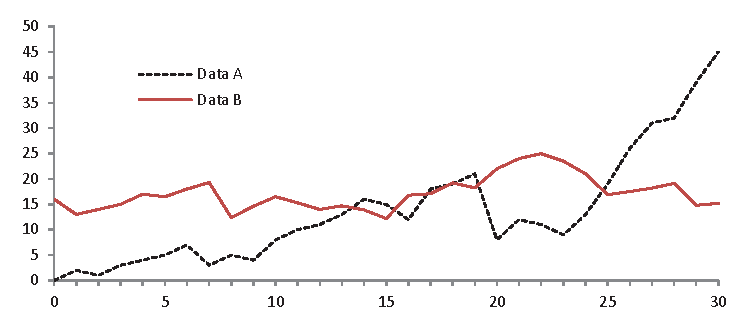
\includegraphics[width=\textwidth]{fig1.eps}
% \caption{A figure caption is always placed below the illustration.
% Please note that short captions are centered, while long ones are
% justified by the macro package automatically.} \label{fig1}
% \end{figure}
%
% \begin{theorem}
% This is a sample theorem. The run-in heading is set in bold, while
% the following text appears in italics. Definitions, lemmas,
% propositions, and corollaries are styled the same way.
% \end{theorem}
% %
% % the environments 'definition', 'lemma', 'proposition', 'corollary',
% % 'remark', and 'example' are defined in the LLNCS documentclass as well.
% %
% \begin{proof}
% Proofs, examples, and remarks have the initial word in italics,
% while the following text appears in normal font.
% \end{proof}
% For citations of references, we prefer the use of square brackets
% and consecutive numbers. Citations using labels or the author/year
% convention are also acceptable. The following bibliography provides
% a sample reference list with entries for journal
% articles~\cite{ref_article1}, an LNCS chapter~\cite{ref_lncs1}, a
% book~\cite{ref_book1}, proceedings without editors~\cite{ref_proc1},
% and a homepage~\cite{ref_url1}. Multiple citations are grouped
% \cite{ref_article1,ref_lncs1,ref_book1},
% \cite{ref_article1,ref_book1,ref_proc1,ref_url1}.

% \subsubsection{Acknowledgements} Please place your acknowledgments at
% the end of the paper, preceded by an unnumbered run-in heading (i.e.
% 3rd-level heading).
%
%
% ---- Bibliography ----
%
% BibTeX users should specify bibliography style 'splncs04'.
% References will then be sorted and formatted in the correct style.

\bibliographystyle{splncs04}
\bibliography{hanging-bib}


\end{document}
